\section{Traceability Survey method } \label{sec:survey}
\begin{figure*}[t]
	\centering
	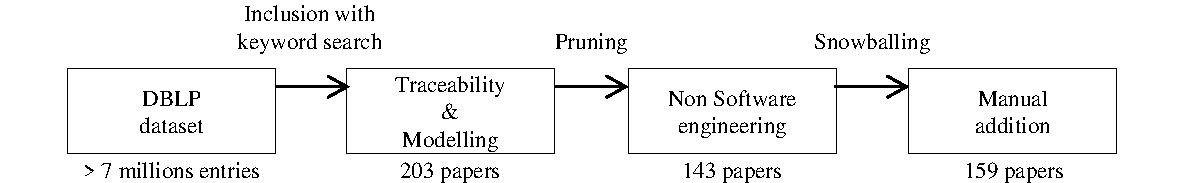
\includegraphics[width=.9\linewidth]{images/survey-process}
	\caption{Survey Process. }
	\label{fig:surveyprocess}
\end{figure*}

In this section we depict the methodology we followed to collect papers proposing traceability solutions, including at the very least the core \textit{representation} component (see previous section). The analysis of these papers will give rise to the feature model we will present next.

The selection process combined the manual selection of a few approaches based on our own experience working in this field and on the works covered by other meta-studies  \cite{Gotel2012,antoniol2017-traceability-grand-challenges,clelandhuang2014-traceability-trends-and-futurte-direction,guo2017-semantically-enhanced-tracebility-deep-learning} together with a systematic literature search by mining bibliographic data sources following the literature review process established by Kitchenham and Charters~\cite{kitchenham2008}. \Fig{fig:surveyprocess} depicts the three main steps of the process.

\subsection{Data source and search strategy}
We used DBLP (2020-07-01~\cite{dblp}) as our core electronic database to search for primary studies on traceability.
To avoid missing possibly relevant approaches, we decided not to put a specific period constraint for the search, but we limited the scope of the search to paper of five pages or more to avoid opinion and vision papers, posters, tool demos and other types of short papers to reduce the number of results while maximizing their quality.

Based on the topic of this survey, we defined the terms of the search query according to the recommendations of Kitchenham and Charters~\cite{kitchenham2008}. We apply the query on the title and abstract of potential relevant publications. As using very generic terms like ``trace'' or ``traceability'' returned thousands of results, we decided to combine in the search query trace-related keywords with language-related ones since any traceability proposal should discuss how traces need to be represented. As many traceability languages are model-based, as part of the language variations we included model, modeling and other core MDE concepts. This brought down the results to 203 papers. 

%Nevertheless, this resulted in too large a number of results with 1100 papers matching the query. Potential papers, at first sight, consisted in a vast majority of false positives. Indeed, "Model" is used in too many fields, "traces" as well, and papers related to software engineering were scarce.
%Since we are not necessarily interested in publications figuring concrete applications of traceability but rather modelling (in a broad sens) work on traceability, we narrowed the scrutiny of the search to work on traceability (modelling tracing) only and we refined once more our query with "traceability", "traces", and "tracer" instead of "trace" for a selection of 771 papers.
%Therefore, we refine the query including keywords more akin to modeling and software engineering, focusing on papers mentioning traceability and not just trace and "modeling" (and its variations and related concepts: "language", "DSL", "transformation", "MDA", "MDD"). This refinement brought down the selection of 203 papers. 

Here is the exact query we applied:
%\begin{verbatim}
	\texttt{.*(([Tt]rac(eability|ing))|([Tt]race[rs])).* AND
	.*(([Mm]odel[- ])(([Dd]riven)|([Bb]ased))| 
	MD[DAE]|Model[l]ing|[Tt]ransformation| DSL|[Ll]anguage).*}
%\end{verbatim}


\subsection{Pruning}
In what follows we describe our inclusion and exclusion criteria. We further explain how we applied these criteria on the previous set of papers. 

\textit{Inclusion criteria}
\begin{enumerate}
	\item the paper is a technical contribution 
	\item the paper is about tracing in software engineering
	\item traceability is the main concern of the paper
\end{enumerate}

\textit{Exclusion criteria}
\begin{enumerate}
	\item the paper is not a primary study
	\item the paper is not a white paper
\end{enumerate}

Before we applied these criteria on the potential papers fetched by our query, we removed automatically papers of less than 5 pages long.
We also automatically extracted papers whose titles mentioned "biology", "education", "kinetics", "logistics", "physiology", "physics", "neuroscience", "agriculture", and "food" which appeared each in a couple of results.  We manually examined the 183 papers left and excluded 40 papers that did not fulfilled the criteria or were duplicates.
% for a remaining total of 123.

\subsection{Snowballing}
At the end of the previous steps, we double-checked that we did not miss any potentially relevant approach due to a number of reasons, \textit{e.g.}, some workshop papers are only indexed by ACM or papers that may be using different synonyms to traceability like ``composition'' or ``extension''. 

Finally, we added papers we were aware of (if not already in the resultset) and a few more we found by snowballing on the selected papers references. They amount to a total of 10 papers. We also manually added the papers of a specific event on traceability, the ECMFA workshop on traceability (\ie ECMFA-TW). 

This lead to a final result of 159 papers. Among them, there are 41 journal articles, 82 in conference proceedings, and 36 workshop reports (see Table \ref{tab:classification-tm}).
\Fig{fig:publicationyears-tm} shows the chronological distribution of the selected publications.


\begin{figure}[h]
	\centering
	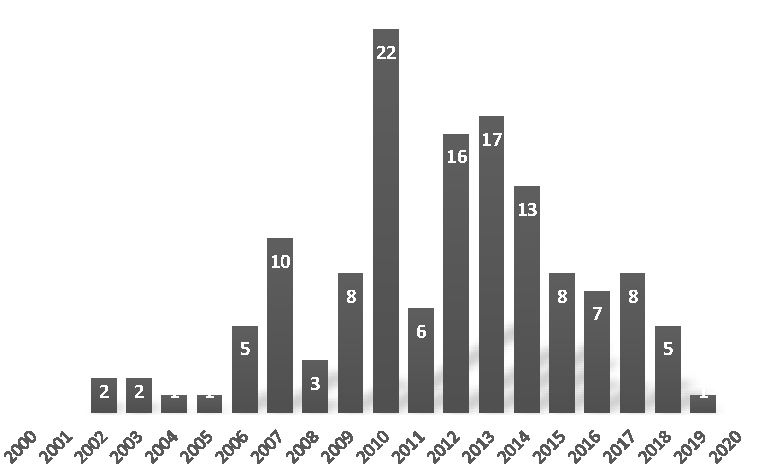
\includegraphics[width=.9\linewidth]{images/publicationyears-tm}
	\caption{Papers selected related to traceability and modeling. }
	\label{fig:publicationyears-tm}	
\end{figure}

\begin{table}[h]
	\centering
	\begin{tabular}{|ll|}
		\hline
		\multicolumn{2}{|l|}{\textbf{Publication type}}  \\ \hline
		\multicolumn{1}{|l}{Journal}          & 41       \\ \hline
		\multicolumn{1}{|l}{Conference}       & 82       \\ \hline
		\multicolumn{1}{|l}{Workshop}         & 36       \\ \hline
	\end{tabular}
	\caption{Publication types of the selected papers.}
	\label{tab:classification-tm}
\end{table}



\subsection{Threats to validity in the selection process}
We acknowledge limitations in the execution of our survey method. 
First, we only used DBLP as a source database. Yet, it is recognized as a {representative} electronic database for scientific publications on software engineering and already contains more than five million publications from more than two million authors.
Setting the limit based on the number of pages alone to elude short papers is another threat to validity. Yet, it is a reproducible practice that limits the number of papers to analyse and thus helps concentrate on the topic rather than the engineering of the survey. 
Finally, the vocabulary related to traceability is scattered among various fields of application with their respective nuances. We mitigate the risk of missing papers by manually adding papers that were not using variations of this term but were still referenced by papers that did. Still, focusing on traceability as a key term was also a conscious decision as we wanted to characterize the works in this field, focusing on those papers that define themselves as part of it. 


%\textbf{Insert some \textbf{statistical distribution} (MM/Meta/concrete application | Modelling traceability vs Tracing modelling | identification of traces | Req. vs other | unstructured text vs others (code, or design model))...}
%63 papers are related to requirement traceability (tracing requirements to other software artefacts).
%8 Meta studies
%76 approaches presenting a language or a framework, and 41 explicitly describing a metamodel.
%22 approaches to trace identification with IR techniques
%22 target source code
%51 target model-level artefacts maintenance and understanding
%





